\documentclass[a4paper,12pt,oneside]{book} 
\usepackage{titlesec}

\titleformat{\chapter}[display]
  {\normalfont\bfseries}{}{0pt}{\Large}

\begin{document}

	
	\pagestyle{empty}\centering
	\textsc{\Large Software Engineering 2 Project\\}
	\textsc{Requirements Analysis and Specification Document}
	\vfill
	\textbf{\Huge PowerEnJoy}
	
	\vfill
	\textsc{\Large Team: Nico Montali, Enrico Fini}
	
	\tableofcontents

	\begin{flushleft}
	\chapter{Introduction}\label{cap:Intro}
	\section{Description of the problem}
We are to project and develop a car-sharing system, PowerEnJoy. This service only relies on electric cars, so more attention is paid to the driver behaviour to reduce infrastructure cost, minimizing the number of necessary charging stations. The system has to interact primarily with the users that want to rent the car, but also with "\textbf{workers}", employees of the company PowerEni, that are responsible for the management of cars themselves. All the cars in the system are connected to the internet through a mobile data receiver and are equipped with several sensor (GPS, speedometer). The system must also provide an \textbf{administration console}, accessible by few users inside PowerEni company. This console provides administration functionalities (e.g. registering new workers, log the state of all the vehicles) and business statistics (e.g. users per day, total driven km). The main users of the system are\\
\begin{description}
\item [User] Users interact with the system primarily through a mobile application, given that users usually rent cars while they are on the move. The application allows users, or "\textbf{drivers}", to reserve a car by presenting a list or map of all the near-by available cars (using the user GPS position). The application allows the user to effectively use the car (find where it is parked, open the doors, find useful informations, e.g. near-by charging stations). The system also provides a web portal, where the user can manage all his informations (payment settings, license, birthdate, view payment history etcetera). Users can access the system only through a registration, that can be done both on the web portal and on the mobile application. During the registration, the user need to provide payment informations and a valid driving license. 
\item [Workers] Workers interact with the system through a specific mobile application, released only to them. Workers are paid by the company to execute "tasks", that include:
\begin{itemize}
\item Recharging on-site a car that was not left in a charging station
\item Move cars to more popular places to maximize usage
\item Pick up a car in the case of an accident or normal maintenance
\end{itemize}

\item [Administrator] Interact with the system through a web application. Given that this is a main asset for the company, because it can effectively block the system, the security of this web application should be very high: possibly a web application accessible only inside PowerEni network with a 2 factor authentication. Once logged in, the administrator can perform these operations
\begin{itemize}
\item Register a new worker newly employed in the system, generating a username and a password (and unregister them)
\item View the status of a single car (e.g. position, battery charge) and request exceptional tasks on it (not the ones generated automatically by the system)
\item View statistics of the system to make better business decisions
\end{itemize}

\end{description}

\section{Goals}
\textbf{Drivers goals}
\begin{itemize}
\item \textbf{[GOAL1]} Log in the system.
\item \textbf{[GOAL2]} Allow drivers to reserve a car up to one hour before they pick it up
\item \textbf{[GOAL3]} Allow drivers to open the reserved car
\item \textbf{[GOAL4]} Allow drivers to pay correctly for the service
\item \textbf{[GOAL5]} Allow drivers to cancel a reservation
\end{itemize}

\textbf{Workers goals}
\begin{itemize}
\item \textbf{[GOAL50]} Log in the system
\item \textbf{[GOAL51]} Dispatch tasks to workers
\item \textbf{[GOAL52]} Allow workers to get informations about an assigned task
\item \textbf{[GOAL53]} Allow workers to open and control the assigned car
\item \textbf{[GOAL54]} Allow workers to keep track of the state of the task (assigned, in progress, done)
\end{itemize}

\textbf{Administrator goals}
\begin{itemize}
\item \textbf{[GOAL100]} Log in the administration console 
\item \textbf{[GOAL101]} Allow to register new workers
\item \textbf{[GOAL102]} Allow to view the status of a specific vehicle
\item \textbf{[GOAL103]} Allow to request an exceptional task on a specific vehicle
\end{itemize}

\section{Domain assumptions}
\begin{itemize}
\item Every car is equipped with some wireless communication system to connect it the the internet.
\item Every car is equipped with GPS, speedometer, passenger presence sensors, engine state sensors, data is sent remotely to the system through the internet.
\item Every car is equipped with a remotely controllable locking system.
\item Every car is legally usable on public street (insurance, taxes, maintenance)
\item Every time the user reserves a car, the payment is pre-authorized by an amount equal to the rent of a day [MAYBE SHOULD NOT BE WRITTEN HERE]
\item Workers are registered in the system by the company itself. The worker application is only distributed to them not on public stores.
\item Every user can reserve a car at a time.
\item Every worker must have only one task assigned at a time.
\item Drivers always respect the driving rules and are able to drive.
\item Driver-provided license informations are assumed to be truthful
\item Safe areas are considered already defined by the management system.
\end{itemize}

\section{Glossary}
\begin{description}
\item [Driver] Client of the system, i.e. the one that uses the service, reserves and drives. Every Driver must provide personal informations (name, surname, email, birthdate, a valid license and payment information.
\item [Ride] A single usage of the service, starts when the user turn on the engine, stops when the car is locked inside a Safe Area;
\item [Blocked driver] A driver that has an invalid license or invalid payment coordinates
\item [Worker] Employee of the company, perform physical actions (moving, charging etc) on cars
\item [Report] Car issue reported by the Driver during a Drive. Will later be assigned to a Worker.
\item [Task]�Piece of work assigned to a worker. Different type of tasks are described later. Every task assigns a single car to a single worker. 
\item [Administrator] Employee of PowerEni that is in charge of the administration of the system through the administration console.
\item [Drop off] The act of leaving the car inside a safe area. This ends the service provided to the driver and effectively make the driver pay
\item [Safe Area] An area in which the Driver can park the car and stop the Service. 
\end{description}

\section{Stakeholders}
The stakeholder is the PowerEni company, who needs the system to provide the service itself.  
\section{References}

	\chapter{Actors}\label{cap:Actors}
	The principal actors involved in the system are
\begin{description}
\item [Driver] Drivers are the main users, external to the PowerEni company, that want to use the PowerEnJoy service. They need to register to the service providing all the needed informations (payment settings and licenses to drive) through the application or the website. 
\item [Worker] Employee of PowerEni, registered by the company itself through the administration console
\item [Administrator] Person inside PowerEni that has access to the administrator console. 
\end{description}
	\chapter{Requirements}\label{cap:Requirements}
	\section{Functional Requirements}

Given all the assumptions, domain properties and constraints from \underline{\autoref{cap:Intro}}, these functional requirements can be stated, listed by the goal they fulfill

\begin{itemize}
\item \textbf{[GOAL1]} Driver must log in the system 
	\begin{itemize}
	\item The system must check if the provided user exists and if the provided password matches
	\item The system must provide further access only if the user is logged
	\end{itemize}
\item \textbf{[GOAL2]} Allow drivers to reserve a car up to one hour before they pick it up
	\begin{itemize}
	\item The system must access driver GPS position or use a user-provided position to recommend the best vehicle to choose
	\item The system must check if the user is logged in and if it is not a blocked driver
	\item The system must check that the user has no other active reservation 
	\item The system must check payment service by pre-authorizing a payment of a fixed amount (to be defined)
	\item The system must reserve the chosen vehicle, i.e. no other user is allowed to reserve the car until it is available again, once the payment is done. The vehicle is considered available again in case of: drop off, cancel registration, one hour passed from the reservation without any driver interaction
	\end{itemize}
\item \textbf{[GOAL3]} Allow drivers to open the reserved car
	\begin{itemize}
	\item The system must check if the user is nearby the reserved car to open it
	\item The system must be able to open the car remotely, only if the user effectively reserved it and is nearby
	\end{itemize}
\item \textbf{[GOAL4]} Allow drivers to pay correctly for the service
	\begin{itemize}
	\item The system must log the whole drive by the driver (elapsed time, driven km)
	\item The system must compute the amount the driver must pay for the service
	\item The system must request a payment of the correct amount 
	\end{itemize}
\item \textbf{[GOAL5]} Allow drivers to cancel a reservation
	\begin{itemize}
	\item The system must be able to cancel a reservation if the driver asks it, given that the reservation has not exceed the 1 hour limit, without making him pay
	\end{itemize}
\item \textbf{[GOAL50]} Worker must log in the system
	\begin{itemize}
	\item The system must check if the provided worker id exists and if the password matches
	\item The system must provide further access only to logged workers
	\end{itemize}
\item \textbf{[GOAL51]} Dispatch tasks to workers
	\begin{itemize}
	\item The system must be able to create a new task. The new task can be created from the administration console or generated automatically by a set of pre-defined rules (e.g. maintenance, usage balance)
	\item The system must select the nearest available worker and assign him the task
	\item The system must notify to the selected user that a new task has been assigned to him
	\end{itemize}
\item \textbf{[GOAL52]} Allow workers to get informations about an assigned task
	\begin{itemize}
	\item The system must provide through the PowerEniWorker App all the needed information for the Worker. These include the GPS position of the car, the reported issue and additional information the user could have provided
	\end{itemize}
\item \textbf{[GOAL53]} Allow workers to open and control the assigned car
	\begin{itemize}
	\item The System, during the assignment of a Task, gives to the chosen Worker the complete control of the car, i.e. normal actions (turn on/off engine, lock/unlock) but also priviliged actions (open hood, access maintenance interfaces, e.g. OBD)
	\end{itemize}
\item \textbf{[GOAL54]} Allow workers to update the state of the task (assigned, in progress, done)
	\begin{itemize}
	\item The System must provide, through the PowerEniWorker App, buttons to change the state of the assigned Task, also with an optional description. Task can be completed or unfixable.
	\end{itemize}
\item \textbf{[GOAL100]} Log in the administration console
	\begin{itemize}
	\item The system must check if the provided Admin ID exists and the password matches
	\item The system must provide further access only to logged Admins
	\end{itemize}
\item \textbf{[GOAL101]} Allow to register new workers
	\begin{itemize}
	\item The System must provide a form to fill in the Admin Portal to insert all the information of the new Worker
	\item The System must create a new Worker account once the previous information are provided.
	\item The System must print the badge used for Worker authentication with the unique Worker signature on it.
	\end{itemize}
\item \textbf{[GOAL102]} Allow to view the status of a specific vehicle
	\begin{itemize}
	\item The System must provide an interface to select a car among all.
	\item The System must provide analytics and current status of the chosen car.
	\end{itemize}
\item \textbf{[GOAL103]} Allow to request an exceptional task on a specific vehicle
	\begin{itemize}
	\item The System must provide an interface to select a car among all.
	\item The System must provide a button to create a new Task, along with specification of the Task itself, inserted manually by the Admin.
	\item The System assigns the newly generated Task to the most suitable available Worker as in a normal Task
	\end{itemize}
\end{itemize}



\section{Non-functional requirements}

\subsection{Usability}
The target user for the service is heterogeneous. It ranges from students, who have a deep understanding of technology, to senior citizens, who find it more difficult. Hence the user interface should be simple and understandable for everyone. \\

\subsection{Privacy and Security}
The system should be able to protect users' personal data, in particular login credentials, payment information and location of the Drivers, which are sensible information nowadays. At the same time we need to find a trade-off between security of our assets (cars and vans) and accessibility for the final user. Therefore our goal is to develop a vulnerability free System using good programming practices. \\

\subsection{Architectural consideration}
The fundamental part of the system is obviously the server-side application, that provides API to interact with the System. 
This server-side application will be written in NodeJS and will use a PostgreSQL DB to store and retrieve data. This application will be deployed on Amazon AWS, in a replicated, distributed and load-balanced way (to grant availability, fault tolerance, scalability), with the DB on a dedicated cluster of servers. 
Three endpoints will be provided, for the 3 categories of user that the System has: an endpoint for the Drivers, one for the Workers and one for the Admins. The Admin endpoint, for security reasons, will only be accessible from the inside PowerEni network (setting AWS firewall rules). 
The web-portal (both for the Driver and for the Admin), will be provided by the same server-side application: it will be built using EJS templates inside NodeJS and JS for client-side scripting. 
The mobile applications, both for Drivers and Workers, will be built natively for iOS, Android and Windows Phone. This applications will communicate with the backend using JSON format.\\

\newpage
\subsection{Mobile application}
\bigbreak
\begin{center}
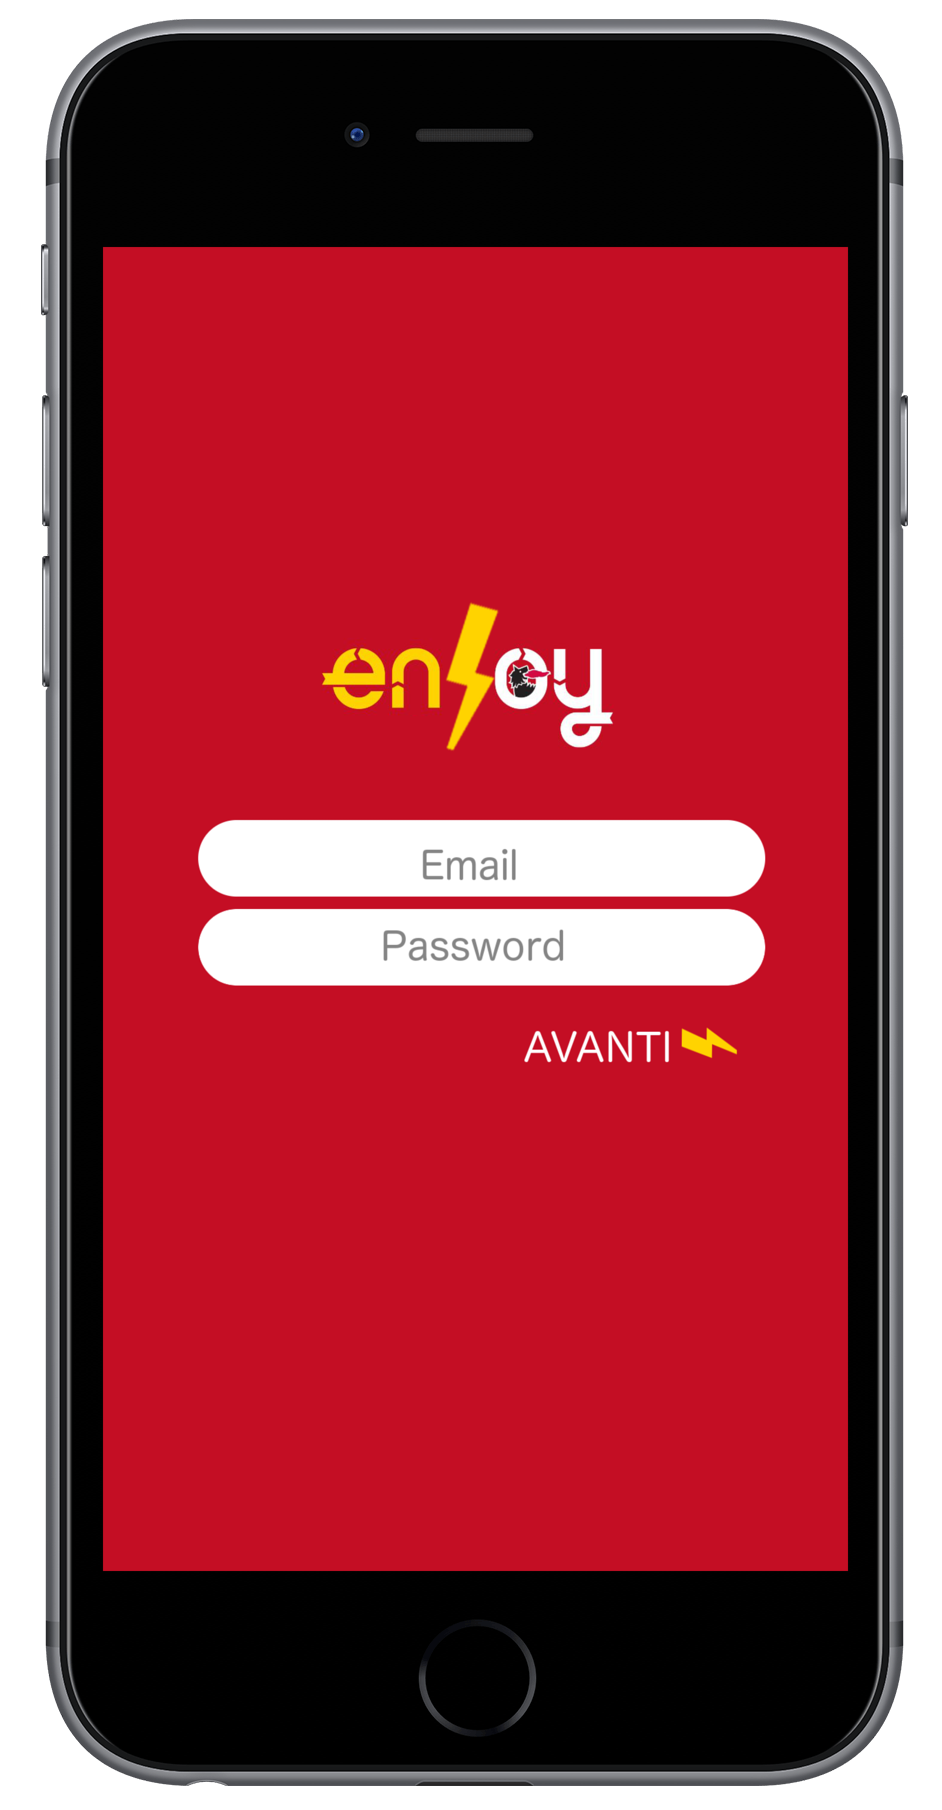
\includegraphics[width=19cm,height=19cm,keepaspectratio]{login}\\
View 1: login
\newpage
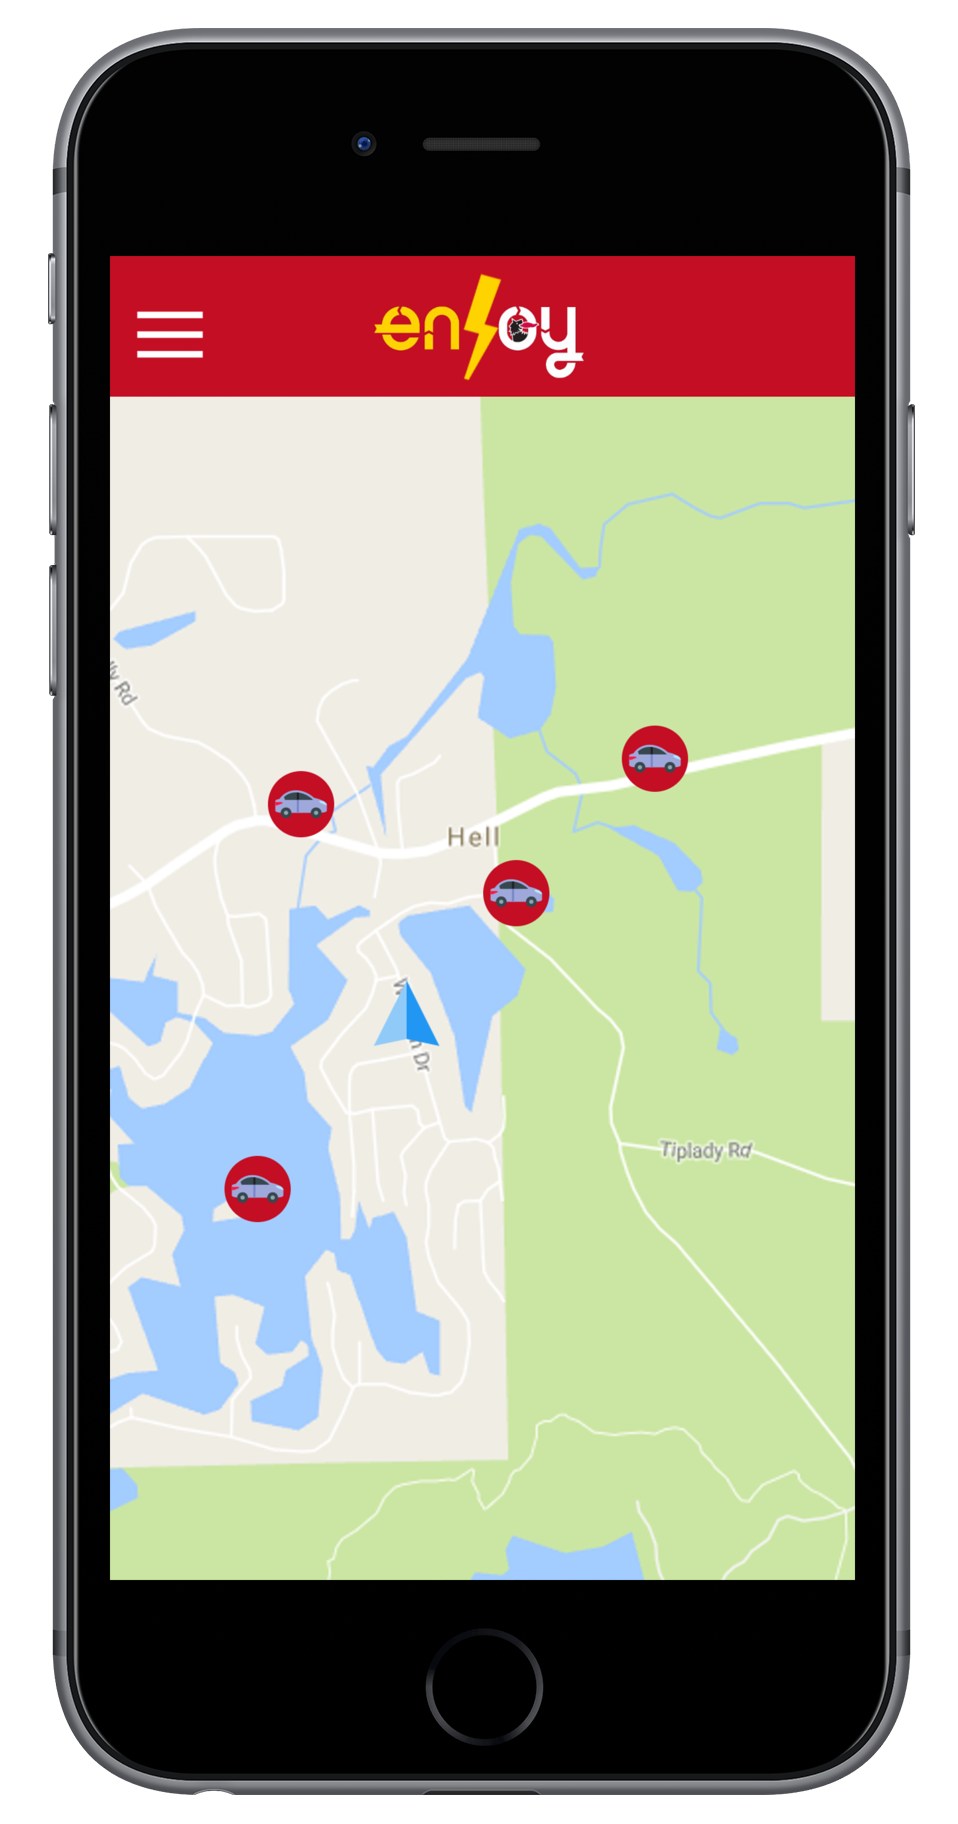
\includegraphics[width=19cm,height=19cm,keepaspectratio]{map}\\
View 2: map
\newpage
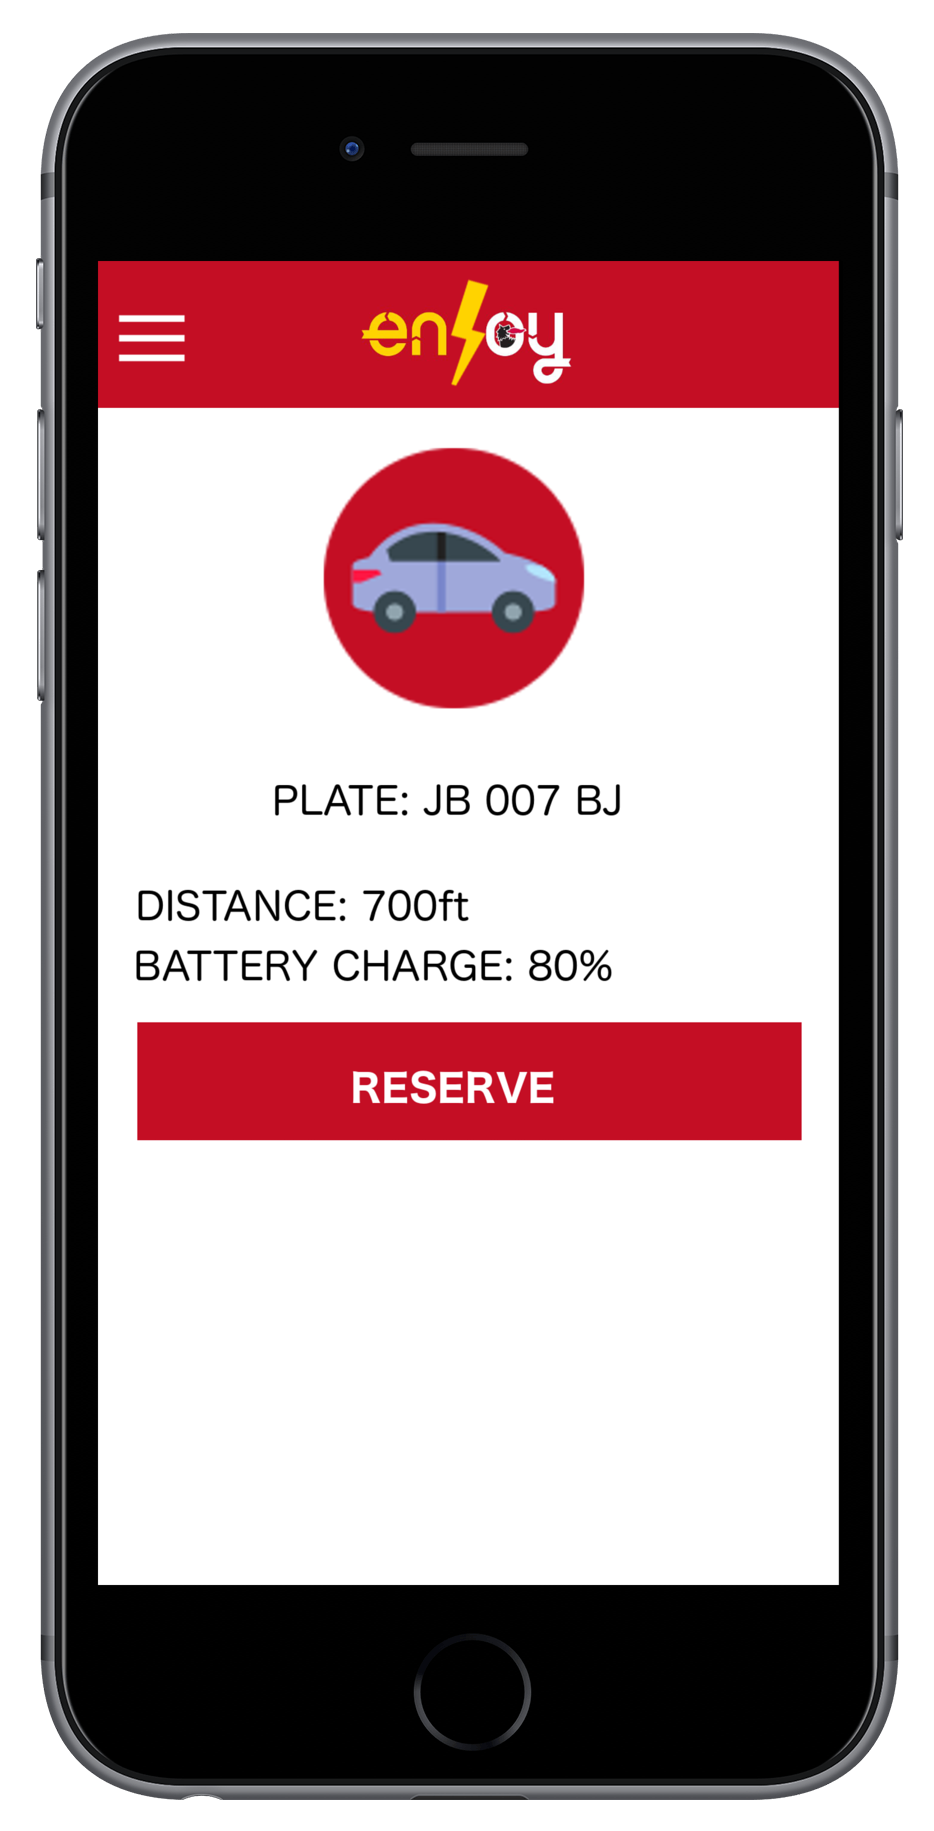
\includegraphics[width=19cm,height=19cm,keepaspectratio]{reserve}\\
View 3: reservation
\end{center}
\newpage

\subsection{Web portal}
\bigbreak
\begin{center}
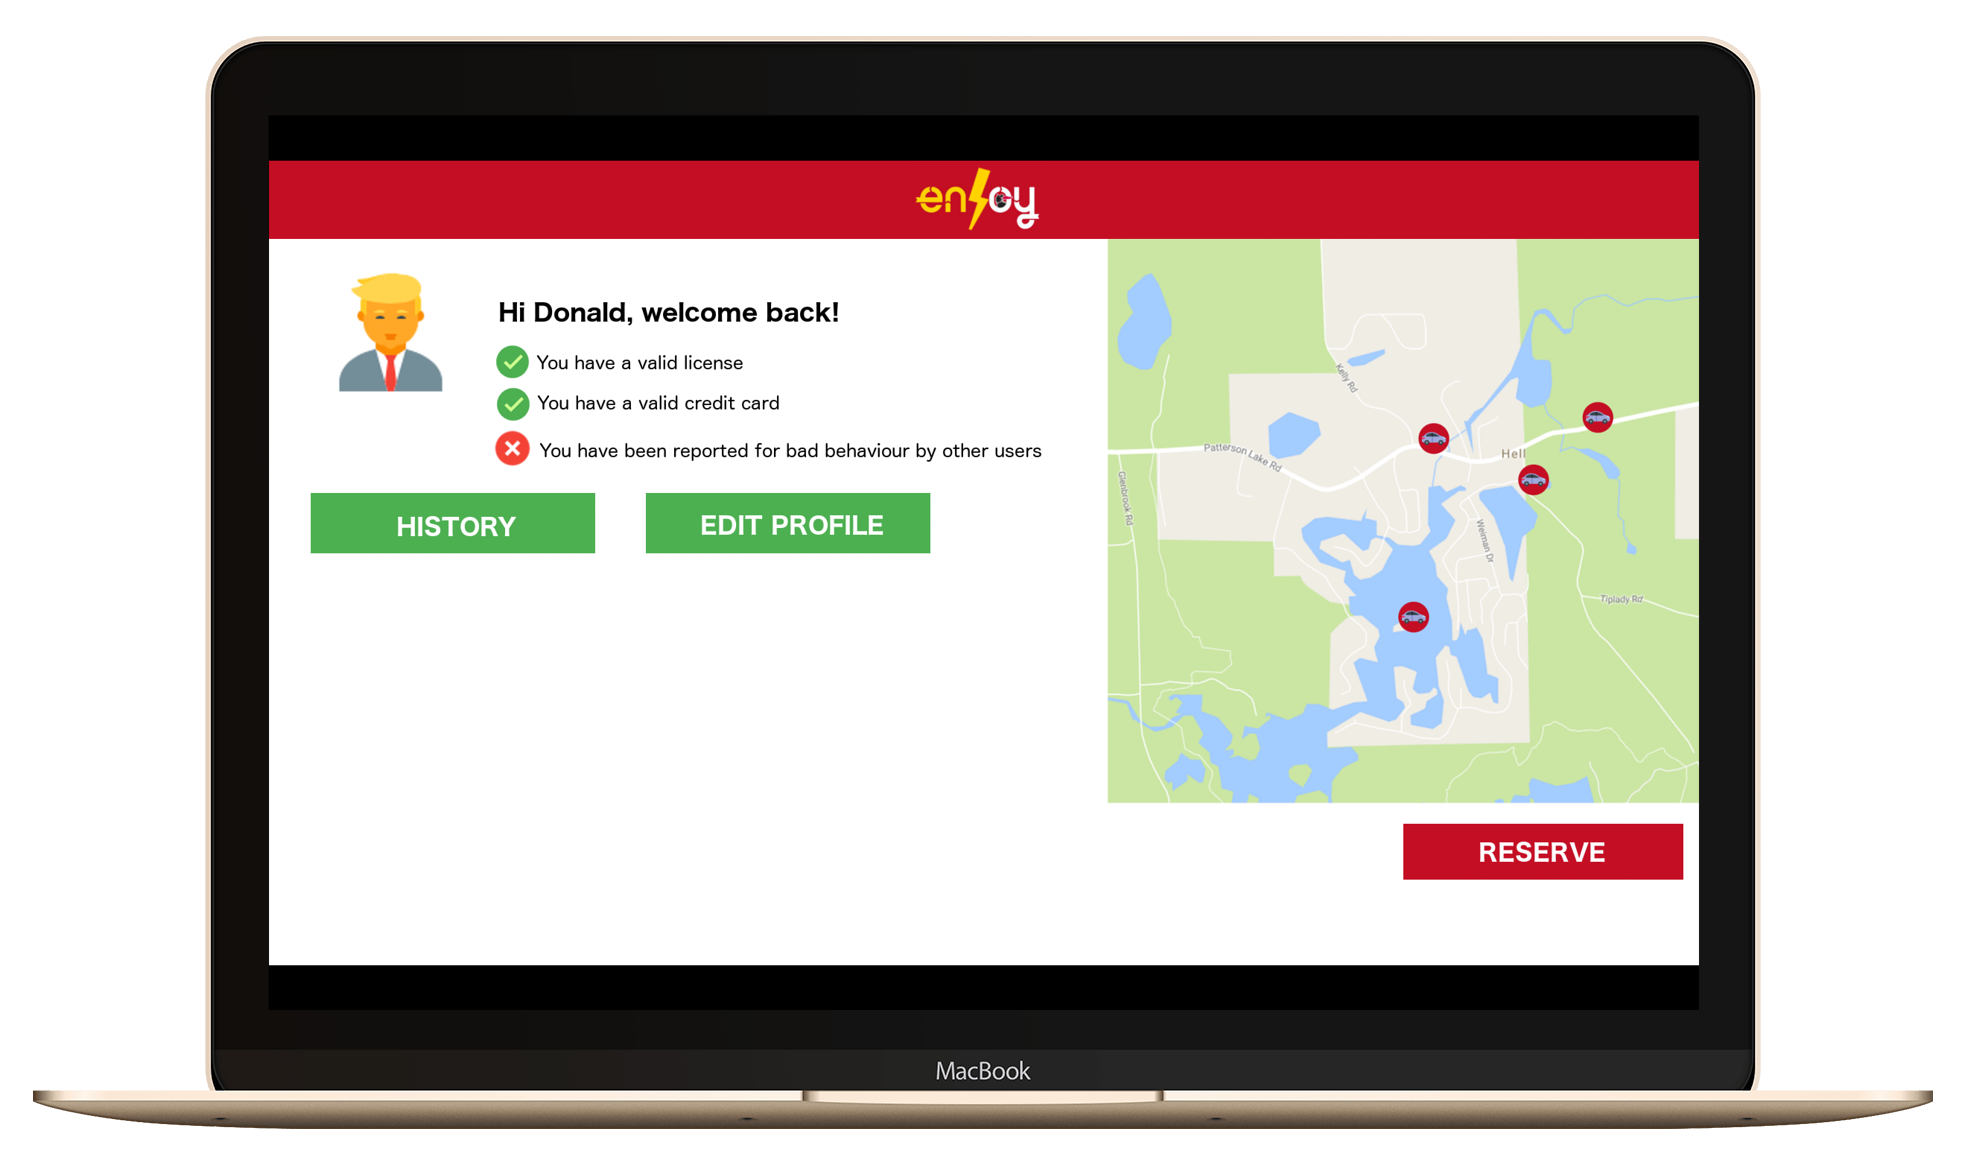
\includegraphics[width=16cm,height=20cm,keepaspectratio]{portal}
Main view
\end{center}





	\chapter{Scenario Identification}\label{cap:ScenarioIdentifying}
	Here we list some possible scenarios of usage of this service:\\
\bigbreak
\bigbreak
\textbf{\large Scenario 1}
\bigbreak
It's about 9 in the morning and Ned, a well-known consultant, is leaving home to go to an important meeting. When he gets in his car and tries to start the engine the car refuses to turn on. Ned is very concerned because the meeting starts at 10 o'clock. Then he remembers of an advertising seen the day before, so he takes out his phone and looks for PowerEnJoy, a new, reliable car sharing service, on the App Store. He is in a hurry but he discovers that the registration mechanism is fast and intuitive. Since the system can recognise and extract information from pictures, he only needs to take a photo of his credit card and driving licence and that's it, few seconds later he is ready to make a reservation using the map of near-by available cars on the application. He is really lucky, the nearest car is only 100m away from his position. When he reaches it he can unlock it directly with his phone. Thanks to this new service Ned managed to arrive on time to the meeting.\\
\bigbreak
\bigbreak
\textbf{\large Scenario 2}
\bigbreak
Anna is a lawyer and every week she must attend some court hearings at the central court of her city. Unfortunately, the central zone of the town has been declared off-limits to traffic to reduce air pollution. Since she is always carrying with her some important documents she cannot use public transport services. Recently she discovered that PowerEnJoy cars, being electric, can enter the city center. Now she uses PowerEnJoy portal every week to find and reserve cars near her house whenever she needs to go to the court for a hearing. Moreover, when she needs to go back home she uses PowerEnjoy application on her Android smartphone. \\
\bigbreak
\bigbreak
\textbf{\large Scenario 3}
\bigbreak
Riccardo is an exchange student who wants to go and see the basketball match at the Arena tonight. Since he has no car he wants to use PowerEnJoy car sharing service to get there. In order to reduce the cost of the ride he decides to pick up some friends on his way. When the new passengers get into the car the seats automatically detect them and the system applies a 10\% discount. When he arrives near the Arena the screen on the car notifies Riccardo the presence of a recharging station close to his position. Hence he decides to park at the station and plug the car to the power station. Then, with his phone, he terminates the rental and the application informs him that he obtained a 40\% total discount. He is really happy with the service and decides to use it also to go back home.\\
\bigbreak
\bigbreak
\textbf{\large Scenario 4}
\bigbreak
Roman is the system administrator of PowerEni. Today, as usual, he is working at PowerEni Headquarter. During his workday he receives a request from the human resources department saying that a new worker, Karim, has been hired. Roman is required to register the new employee in the system. To do that he opens an ad hoc tool on his computer. The tool provides an intuitive user interface for the management of workers' accounts. After having processed the information of the new worker the system prints his new badge and writes a unique NFC signature on it. Few minutes later Karim arrives at the Headquarter and picks up his badge. Then he downloads PowerEniWorker application, creates an account, activates it using the NFC tag and finally registers his fingerprint for future usage. Karim is ready to start working for PowerEni\\
\bigbreak
\bigbreak
\textbf{\large Scenario 5}
\bigbreak
Karim is a worker at PowerEni. At the beginning of his workday he opens his PowerEniWorker application and logs in using either his fingerprint or the NFC signature of his identification badge. Automatically the system marks his status as ``available" and starts computing a suitable personalised task for the worker. Meanwhile, not far away from Karim's position, Alan, a user, is reporting a flat tire on his car using the dedicated button on PowerEnJoy application. The system terminates Alan's rental and marks the car as ``to be repaired". Since Karim is the nearest available worker, the server sends him a push notification with all the information needed to reach and repair Alan's car. Therefore Karim accepts the task, changing his status to ``busy", and gets in his electric van (provided by PowerEni). Once he reaches the faulty car he fixes the flat tire. Finally, always using PowerEniWorker application, he marks the task as ``done". The system reacts assigning a new task to Karim and changing the status of the car to ``available". \\

	\chapter{UML diagrams}\label{cap:UML}
	\section{Use case diagram}
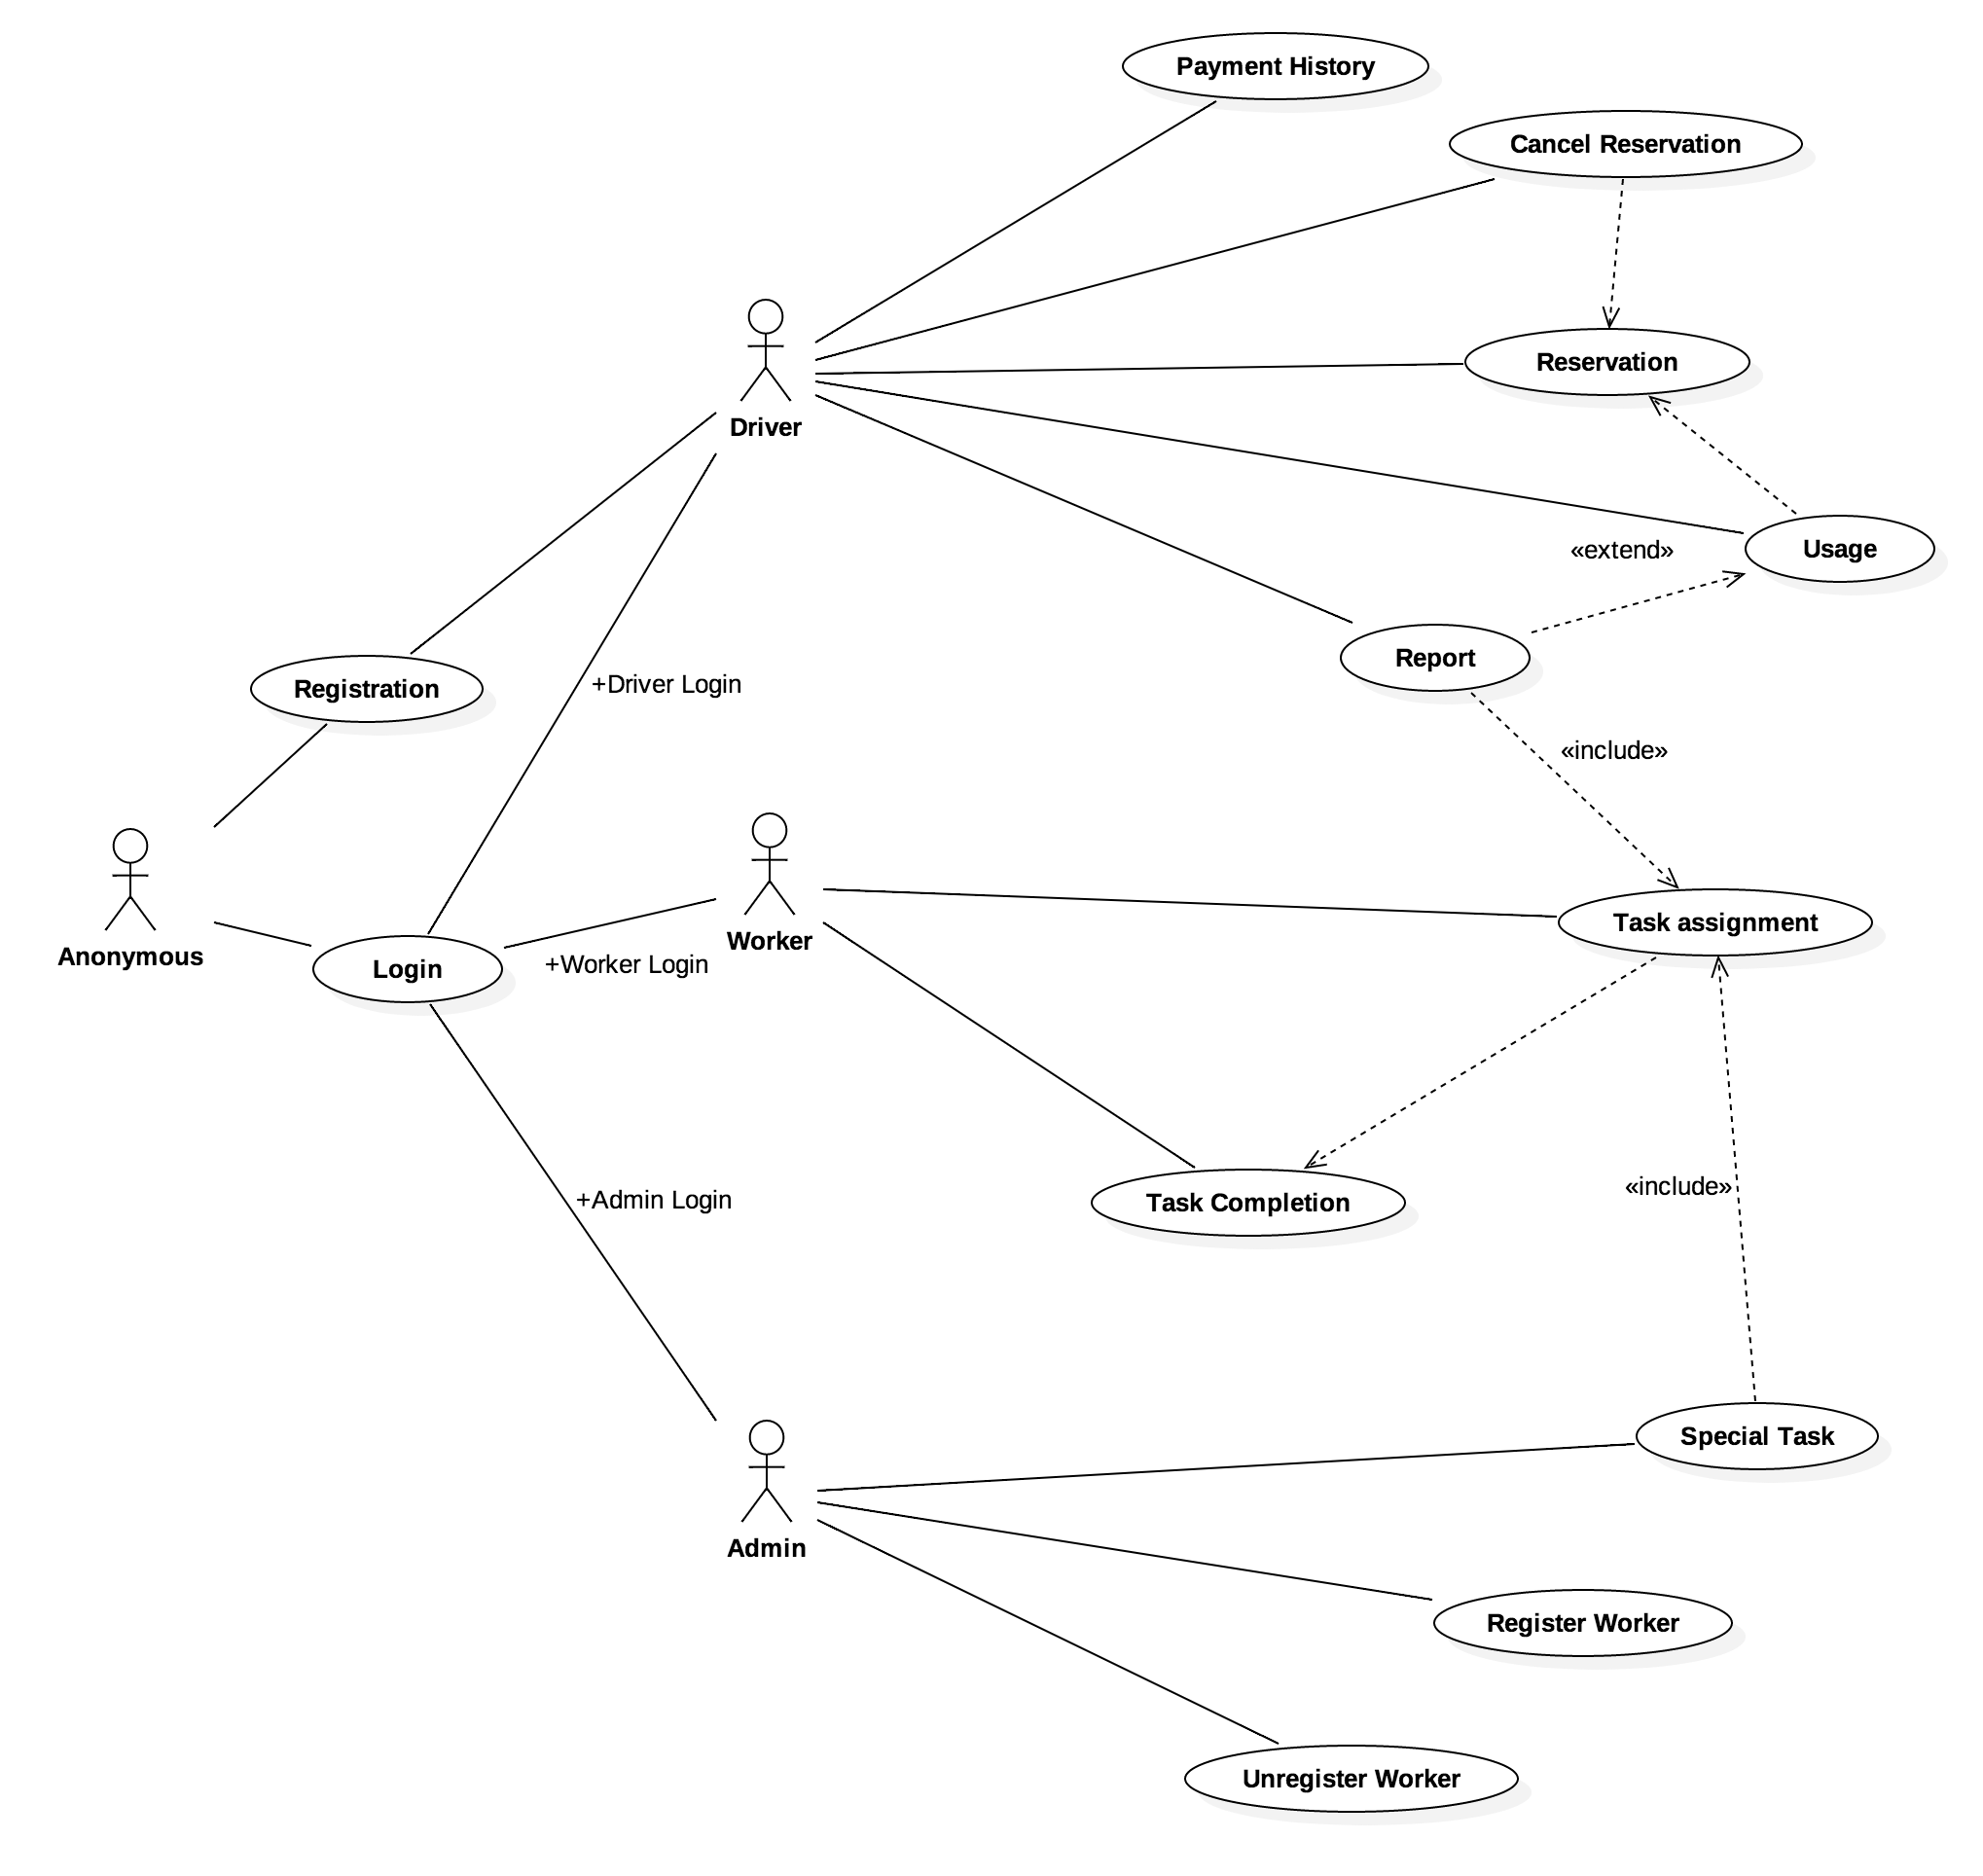
\includegraphics[width=13cm,height=13cm,keepaspectratio]{usecase}
\section{Driver use cases}
Here we list relevant use cases for the Driver:\\
\begin{center}
\noindent\rule{8cm}{1.0pt}
\end{center}

\textbf{\large Driver registration}
\bigbreak
\textbf{Name:} Driver registration \\
\textbf{Actors:} Driver \\
\textbf{Entry conditions:} 
\begin{itemize}
\item The Driver has already downloaded the application or he/she is on the web portal.
\end{itemize}
\textbf{Flow of events:} 
\begin{itemize}
\item The Driver provides an email and a password;
\item The Driver provides information about himself/herself (full name, date of birth, address, sex);
\item The Driver clicks the sign up button;
\item The System verifies if the email is valid and not already in use;
\item The System verifies if the password matches the rules (lenght, special characters);
\item The System asks for driving license and payment information;
\item The Driver uploads pictures of his license and credit card;
\item The System shows a "success" message and sends a confirmation email.
\end{itemize}
\textbf{Exit conditions:} the Driver is registered and logged into the system.\\
\textbf{Exceptions:} 
\begin{itemize}
\item If submitted data is not valid the System asks for them again.
\end{itemize}

\begin{center}
\noindent\rule{8cm}{1.0pt}
\end{center}


\textbf{\large Driver login}
\bigbreak
\textbf{Name:} Driver login \\
\textbf{Actors:} Driver \\
\textbf{Entry conditions:} 
\begin{itemize}
\item The Driver has already downloaded the application or he/she is on the web portal.
\end{itemize}
\textbf{Flow of events:} 
\begin{itemize}
\item The Driver provides username and password;
\item The Driver clicks the login button;
\item The System verifies the credentials.
\end{itemize}
\textbf{Exit conditions:} the Driver is logged into the system.\\
\textbf{Exceptions:} 
\begin{itemize}
\item If credentials are wrong the system asks for them again.
\end{itemize}


\begin{center}
\noindent\rule{8cm}{1.0pt}
\end{center}


\textbf{\large Car reservation}
\bigbreak
\textbf{Name:} Car reservation \\
\textbf{Actors:} Driver \\
\textbf{Entry conditions:} 
\begin{itemize}
\item The Driver is logged in;
\item The Driver must not be a Blocked Driver.
\end{itemize}
\textbf{Flow of events:} 
\begin{itemize}
\item The System automatically fetches the Driver's position and presents a list of available nearby cars;
\item The Driver selects one of the available cars;
\item The System pre-authorizes the fixed amount from the credit card and marks the car as reserved;
\item The System shows a "success" message and sends an email with reservation information (car location, car plate, cancel reservation link)
\end{itemize}
\textbf{Exit conditions:} 
\begin{itemize}
\item The Driver has a reservation and cannot reserve other cars 
\item The car is not available for other Drivers.\\
\end{itemize}
\textbf{Exceptions:} 
\begin{itemize}
\item If the Driver does not have enough money the reservation in not successful.
\end{itemize}


\begin{center}
\noindent\rule{8cm}{1.0pt}
\end{center}


\textbf{\large Driver uses the service}
\bigbreak
\textbf{Name:} Driver uses the service\\
\textbf{Actors:} Driver \\
\textbf{Entry conditions:} 
\begin{itemize}
\item The Driver has already reserved a car.
\end{itemize}
\textbf{Flow of events:} 
\begin{itemize}
\item The System waits till the user is nearby the car then enables the open button on the application;
\item The Driver opens the car by pressing the button;
\item The Driver gets inside the car, turns it on and begins to drive;
\item The System logs the route and the duration of the drive;
\item The System presents to the Driver his current due amount and all the nearby recharging stations;
\item The Driver stops the car, gets outside the car and closes the door;
\item 30 seconds later the car automatically locks itself and the ride is terminated by the System;
\item The System calculates the correct amount to be paid (depending on discount policies) and charges the Driver's credit card accordingly.
\end{itemize}
\textbf{Exit conditions:} the Driver got to the final destination and the car is marked again as "available".\\
\textbf{Exceptions:}  
\begin{itemize}
\item If the Driver does not start his ride within one hour, the reservation expires and his credit card is charged 1 Euro and the car status is reset to "available". 
\end{itemize}

\begin{center}
\noindent\rule{8cm}{1.0pt}
\end{center}


\textbf{\large Cancel reservation}
\bigbreak
\textbf{Name:} Cancel reservation\\
\textbf{Actors:} Driver \\
\textbf{Entry conditions:} 
\begin{itemize}
\item The Driver has already reserved a car;
\item The reservation happened within one hour.
\end{itemize}
\textbf{Flow of events:} 
\begin{itemize}
\item The user clicks either on the "cancel reservation" button on the application or on the "cancel reservation" link provided in the reservation email;
\item The System cancels the reservation without charging the user.
\end{itemize}
\textbf{Exit conditions:} 
\begin{itemize}
\item The car is marked as "available" again;
\item The Driver can reserve cars again.
\end{itemize}
\textbf{Exceptions:} there are no exceptions for this use case.\\


\begin{center}
\noindent\rule{8cm}{1.0pt}
\end{center}


\textbf{\large Report a problem}
\bigbreak
\textbf{Name:} Report a problem\\
\textbf{Actors:} Driver \\
\textbf{Entry conditions:} 
\begin{itemize}
\item The Driver started his ride;
\item The car has a problem.
\end{itemize}
\textbf{Flow of events:} 
\begin{itemize}
\item The Driver clicks on the "report" button and specifies the type of problem; 
\item The ride terminates and the Driver pays accordingly;
\item The Driver gets outside the car.
\end{itemize}
\textbf{Exit conditions:} 
\begin{itemize}
\item A Task is generated and is assigned to the most suitable available Worker;
\item The Driver can reserve cars again.
\end{itemize}
\textbf{Exceptions:} there are no exceptions for this use case.\\


\begin{center}
\noindent\rule{8cm}{1.0pt}
\end{center}



\textbf{\large View payment history}
\bigbreak
\textbf{Name:} View payment history\\
\textbf{Actors:} Driver \\
\textbf{Entry conditions:} 
\begin{itemize}
\item The Driver is logged into the System.
\end{itemize}
\textbf{Flow of events:} 
\begin{itemize}
\item The Driver clicks on the Personal History button inside the web portal
\item The System presents a detailed log of all the previous reservation and payments.
\end{itemize}
\textbf{Exit conditions:} 
\begin{itemize}
\item The Driver is informed on his/her history.
\end{itemize}
\textbf{Exceptions:} there are no exceptions for this use case.\\


\begin{center}
\noindent\rule{8cm}{1.0pt}
\end{center}



\section{Worker use cases}
Here we list relevant use cases for the Worker:\\
\begin{center}
\noindent\rule{8cm}{1.0pt}
\end{center}


\textbf{\large Worker login}
\bigbreak
\textbf{Name:} Worker login \\
\textbf{Actors:} Worker \\
\textbf{Entry conditions:} 
\begin{itemize}
\item The Worker has already downloaded the application;
\item The Worker has been registered by an Admin.
\end{itemize}
\textbf{Flow of events:} 
\begin{itemize}
\item The Worker places the NFC badge on his phone;
\end{itemize}
\textbf{Exit conditions:} 
\begin{itemize}
\item The Worker is logged into the system and his workday begins.
\end{itemize}
\textbf{Exceptions:} there are no exceptions for this use case.\\


\begin{center}
\noindent\rule{8cm}{1.0pt}
\end{center}


\textbf{\large Task assignment}
\bigbreak
\textbf{Name:} Task assignment\\
\textbf{Actors:} Worker \\
\textbf{Entry conditions:} 
\begin{itemize}
\item The Worker is logged into the System;
\item The Worker is available;
\item The System generated a Task which has not been assigned yet.
\end{itemize}
\textbf{Flow of events:} 
\begin{itemize}
\item The System chooses the most suitable available Worker depending on its policies (distance, workload, van batteries);
\item The System notifies with a push notification the selected Worker and sends him all the needed information (location, type of task, car info).
\end{itemize}
\textbf{Exit conditions:} 
\begin{itemize}
\item The Task is assigned to the worker;
\item The Worker is marked as busy.
\end{itemize}
\textbf{Exceptions:} there are no exceptions for this use case.\\



\begin{center}
\noindent\rule{8cm}{1.0pt}
\end{center}


\textbf{\large Task completion}
\bigbreak
\textbf{Name:} Task completion\\
\textbf{Actors:} Worker \\
\textbf{Entry conditions:} 
\begin{itemize}
\item The Worker has been assigned a Task;
\item The Worker completed the task;
\end{itemize}
\textbf{Flow of events:} 
\begin{itemize}
\item The Worker informs the System that the work has been completed using the application;
\end{itemize}
\textbf{Exit conditions:} 
\begin{itemize}
\item The Worker is marked as available again;
\end{itemize}
\textbf{Exceptions:} 
\begin{itemize}
\item If the Worker did not manage to complete the Task he closes the Task providing a description. The System Admin will manage the situation manually (e.g. calling a tow truck).
\end{itemize}


\begin{center}
\noindent\rule{8cm}{1.0pt}
\end{center}


\section{Admin use cases}
Here we list relevant use cases for the Admin:\\
\begin{center}
\noindent\rule{8cm}{1.0pt}
\end{center}


\textbf{\large Admin login}
\bigbreak
\textbf{Name:} Admin login \\
\textbf{Actors:} Admin \\
\textbf{Entry conditions:} there are no entry conditions for this use case.\\
\textbf{Flow of events:} 
\begin{itemize}
\item The Admin provides his credentials to the System  
\end{itemize}
\textbf{Exit conditions:} 
\begin{itemize}
\item The Admin is logged into the System.
\end{itemize}
\textbf{Exceptions:} there are no exceptions for this use case.\\


\begin{center}
\noindent\rule{8cm}{1.0pt}
\end{center}


\textbf{\large Register employee}
\bigbreak
\textbf{Name:} Register employee \\
\textbf{Actors:} Admin \\
\textbf{Entry conditions:} 
\begin{itemize}
\item The Admin is logged into the System.
\end{itemize}
\textbf{Flow of events:} 
\begin{itemize}
\item The Admin provides the new employee's information to the System (full name, ID);
 \item The System prints the new Worker's badge and writes a unique NFC signature on it.
\end{itemize}
\textbf{Exit conditions:} 
\begin{itemize}
\item The new Worker is registered.
\end{itemize}
\textbf{Exceptions:} there are no exceptions for this use case.\\


\begin{center}
\noindent\rule{8cm}{1.0pt}
\end{center}


\textbf{\large Unregister employee}
\bigbreak
\textbf{Name:} unregister employee \\
\textbf{Actors:} Admin \\
\textbf{Entry conditions:} 
\begin{itemize}
\item The Worker has been fired or reassigned.
\end{itemize}
\textbf{Flow of events:} 
\begin{itemize}
\item The Admin selects the employee to be unregistered.
\end{itemize}
\textbf{Exit conditions:} 
\begin{itemize}
\item The Worker is no more registered and his credentials are invalidated.
\end{itemize}
\textbf{Exceptions:} there are no exceptions for this use case.\\


\begin{center}
\noindent\rule{8cm}{1.0pt}
\end{center}


\textbf{\large Get analytics}
\bigbreak
\textbf{Name:} get analytics \\
\textbf{Actors:} Admin \\
\textbf{Entry conditions:} 
\begin{itemize}
\item The Admin is logged in.
\end{itemize}
\textbf{Flow of events:} 
\begin{itemize}
\item The Admin selects the car or the worker to get analytics of;
\end{itemize}
\textbf{Exit conditions:} 
\begin{itemize}
\item The System shows detailed analytics
\end{itemize}
\textbf{Exceptions:} there are no exceptions for this use case.\\


\begin{center}
\noindent\rule{8cm}{1.0pt}
\end{center}


\textbf{\large Request special Task}
\bigbreak
\textbf{Name:} request special Task \\
\textbf{Actors:} Admin \\
\textbf{Entry conditions:} 
\begin{itemize}
\item The Admin is logged in.
\end{itemize}
\textbf{Flow of events:} 
\begin{itemize}
\item The Admin writes a description of the special Task, including the car ID.
\end{itemize}
\textbf{Exit conditions:} 
\begin{itemize}
\item A Worker is notified.
\end{itemize}
\textbf{Exceptions:} there are no exceptions for this use case.\\


\begin{center}
\noindent\rule{8cm}{1.0pt}
\end{center}

	\end{flushleft}

\end{document}